\documentclass[a4paper]{article}

\usepackage{graphicx}
\usepackage{amsmath,amssymb}
\usepackage{minted}
\usepackage{multirow}
\usepackage{float}
\usepackage{algorithm}
\usepackage{algpseudocode}
\usepackage{todonotes}
\usepackage{forest}
\usepackage{xstring}
\usepackage{xcolor}
\usepackage[most]{tcolorbox}
\usepackage{xparse}
\usepackage{natbib}
\usepackage{adjustbox}

\usetikzlibrary{graphs,graphdrawing}
\usegdlibrary{layered}

% for external graphviz
\input{/home/donkarlo/Dropbox/repo/nd_language_ai_project/src/nd_language_ai/formal/computer/programming/tex/latex/code_clips/external_graphviz.tex}

% for tags
\input{/home/donkarlo/Dropbox/repo/nd_language_ai_project/src/nd_language_ai/formal/computer/programming/tex/latex/part/control_sequence/kind/semtag/semtag.tex}

% for links
\input{/home/donkarlo/Dropbox/repo/nd_language_ai_project/src/nd_language_ai/formal/computer/programming/tex/latex/code_clips/seehere.tex}

% for nested lists and sections
\input{/home/donkarlo/Dropbox/repo/nd_language_ai_project/src/nd_language_ai/formal/computer/programming/tex/latex/code_clips/deep_structure.tex}

\title{Language building}
\date{}
\author{Mohammad Rahmani}

\begin{document}
   \maketitle
   \begin{figure}[H]
      \centering
      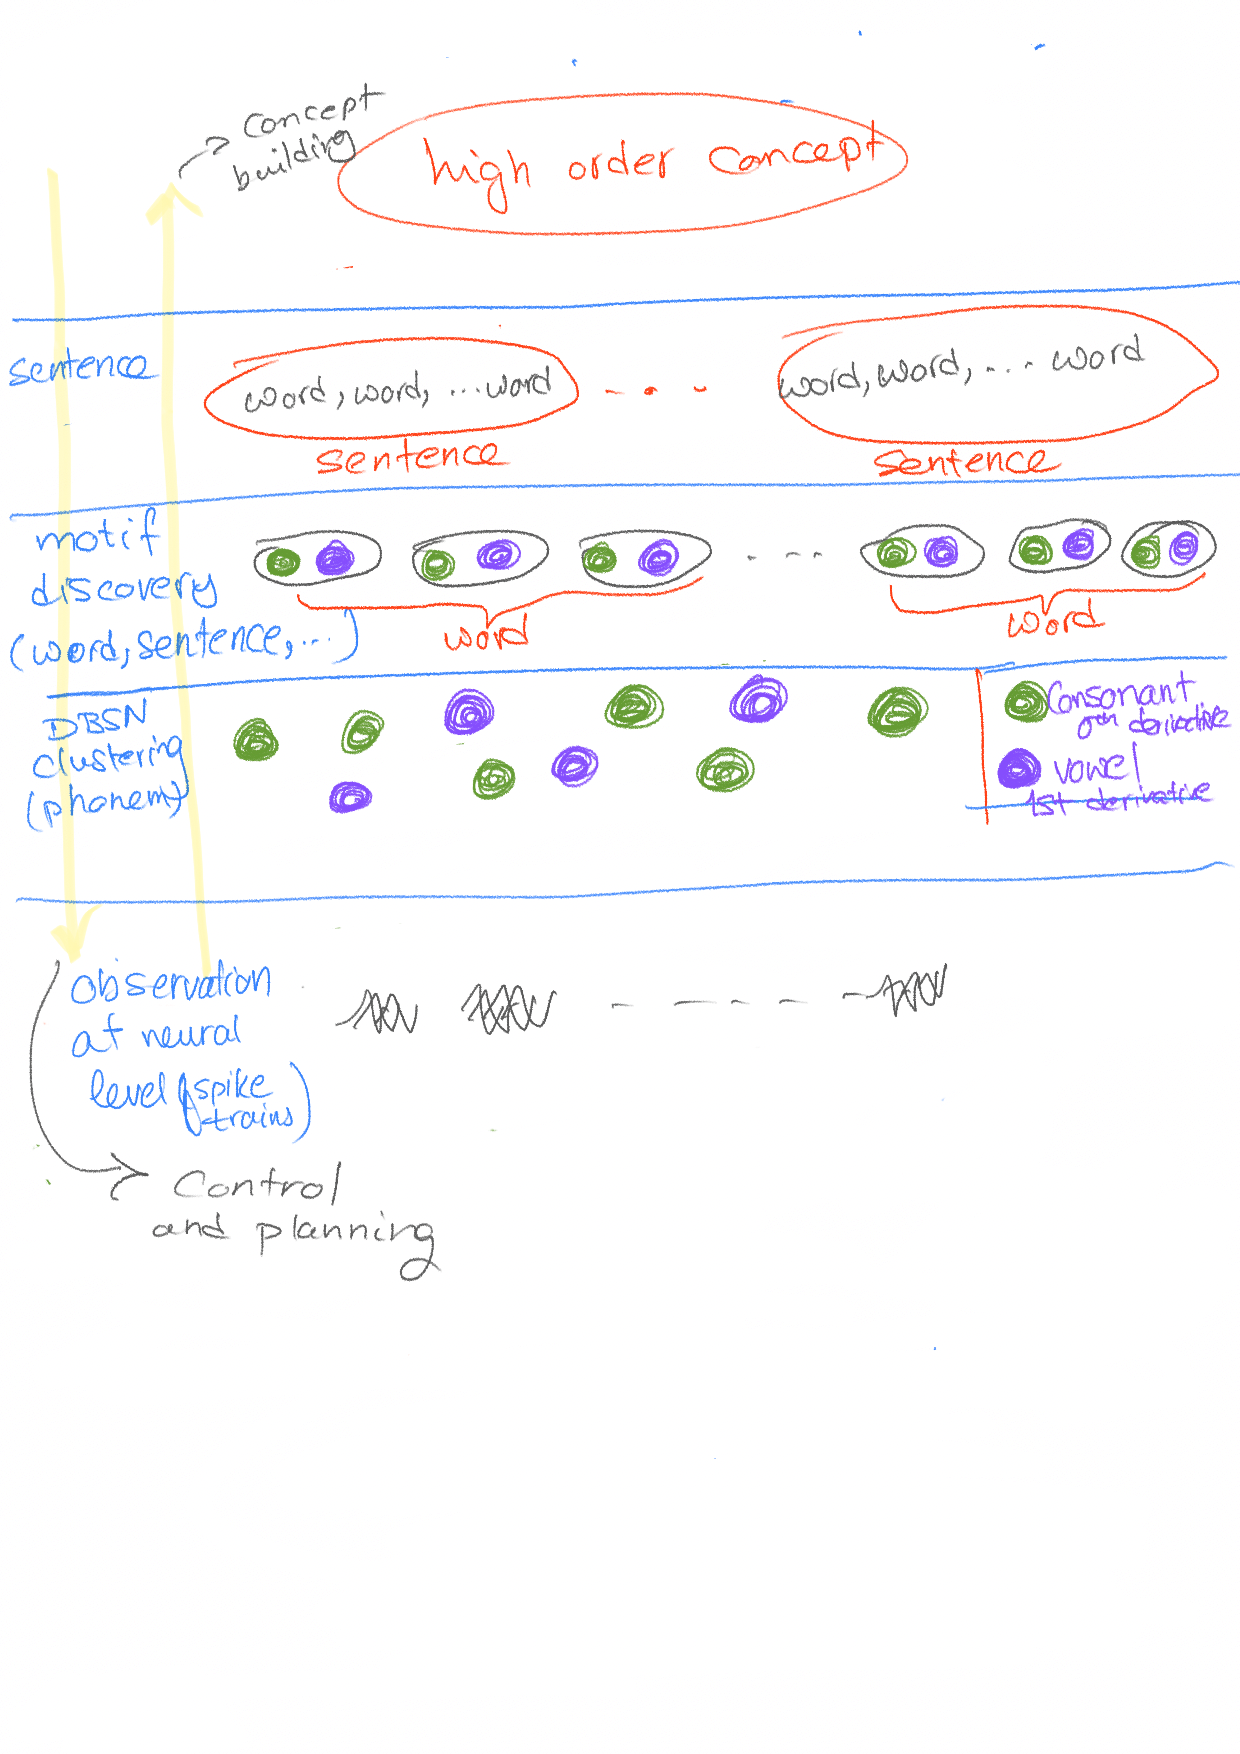
\includegraphics[width=0.9\textwidth]{language_building.png}
   \end{figure}
      \subsection{Motif discovery (to cluster timeseries)}
         In this research Matrix-Profile-based is used to cluster phonems to build words and to higher levels. This is explained in language section .

         \seeherefooter{/home/donkarlo/Dropbox/repo/nd_math_learning_project/src/statistics/sequence/timeseries/motif_discovery/matrix_profile_based/matrix_profiled_based.tex}
         To discover the periodic data. As we will see in the experiment section a drone that circules a rectangualar corridor makes many periodic sensory data that motif discovery is used for it. Then a method is needed to find the cycles in sensory data.

         This research uses Matrix-Profile-based  method for this .

         This method doesn't need training.
         \textbf{Matrix-Profile-based Motif Discovery \cite{vanonsem-2023-variable-length-motif-discovery-in-time-series-data}}
         \begin{algorithm}[H]
            \caption{Event-Driven Variable-Length Motif Discovery}
            \begin{algorithmic}[1]
               \State Input time series \(T\), window size \(w\), threshold \(t\)
               \State Compute scale-aware distance matrix \(M\)
               \State Convert \(M\) to binary event matrix \(M_{\mathrm{bin}}\)
               \State Rank diagonals of \(M_{\mathrm{bin}}\) by number Weightof events
               \For{each ranked diagonal}
               \For{each event on the diagonal}
               \State Enlarge the event into a motif candidate
               \State Validate candidate using the distance threshold
               \State Find all occurrences of the accepted motif
               \State Add motif and its occurrences to output
               \State Exclude found occurrences from \(M_{\mathrm{bin}}\)
               \EndFor
               \EndFor
               \State Return unique motifs with grouped occurrences
            \end{algorithmic}
         \end{algorithm}
         \bibliographystyle{plainnat}
         \bibliography{/home/donkarlo/Dropbox/repo/nd_shared_research/bibliography/bibliography.bib}
\end{document}
